\documentclass[aspectratio=16:9, xcolor=dvipsnames]{beamer}

% Packages
\usepackage[utf8]{inputenc}
\usepackage{graphicx}
\usepackage{tikz}
\usepackage{amsmath}
\usepackage{amssymb}
\usepackage{xcolor}
\usepackage{hyperref}
\usepackage{fontawesome5}
\usepackage{multicol}
\usepackage{listings}

% TikZ Libraries
\usetikzlibrary{shapes, arrows, positioning, fit, shadows, calc}

% Custom Colors
\definecolor{Primary}{RGB}{255, 152, 0}       % Orange
\definecolor{Secondary}{RGB}{41, 88, 255}     % Blue
\definecolor{Accent}{RGB}{76, 175, 80}        % Green
\definecolor{DarkBg}{RGB}{30, 30, 30}         % Dark Background
\definecolor{LightBg}{RGB}{240, 240, 240}     % Light Background
\definecolor{Warning}{RGB}{255, 87, 34}       % Red-Orange

% Theme Customization
\usetheme{Madrid}
\usecolortheme{default}

% Custom Color Scheme
\setbeamercolor{structure}{fg=Primary}
\setbeamercolor{alerted text}{fg=Warning}
\setbeamercolor{block title}{bg=Primary, fg=white}
\setbeamercolor{block body}{bg=Primary!10, fg=black}
\setbeamercolor{title}{fg=Primary}
\setbeamercolor{subtitle}{fg=Secondary}
\setbeamercolor{frametitle}{bg=Primary, fg=white}
\setbeamercolor{section in toc}{fg=Primary}

% Custom Footer
\setbeamertemplate{footline}{
    \hbox{%
        \begin{beamercolorbox}[wd=0.5\paperwidth,ht=2.25ex,dp=1ex,left]{title in head/foot}%
            \usebeamerfont{title in head/foot}\hspace*{2ex}\insertshortauthor
        \end{beamercolorbox}%
        \begin{beamercolorbox}[wd=0.5\paperwidth,ht=2.25ex,dp=1ex,right]{date in head/foot}%
            \usebeamerfont{date in head/foot}\insertframenumber{} / \inserttotalframenumber\hspace*{2ex}
        \end{beamercolorbox}}%
    \vskip0pt%
}

% Title Page Style
\setbeamertemplate{title page}{
    \begin{tikzpicture}[remember picture, overlay]
        % Background gradient effect
        \fill[color=Primary!5] (current page.south west) rectangle (current page.north east);
        \fill[color=Secondary!10] (current page.north west) -- (current page.north east) -- 
              ($(current page.north east)!0.3!(current page.south east)$) -- 
              ($(current page.north west)!0.3!(current page.south west)$) -- cycle;
    \end{tikzpicture}
    
    \vspace*{1cm}
    \centering
    
    % Logo
    \includegraphics[width=0.25\textwidth]{../assets/logo/PICK\ MY\ DISH.png}\\[1.5cm]
    
    % Title
    {\Huge \textbf{\textcolor{Primary}{PICK MY DISH}}}\\[0.5cm]
    {\Large \textcolor{Secondary}{\textit{Your Personal Cooking Companion}}}\\[2cm]
    
    % Subtitle
    {\large \textcolor{DarkBg}{Intelligent Recipe Recommendation System}}\\[3cm]
    
    % Team Information
    {\small \textcolor{Secondary}{\textbf{Team Members:}}}\\
    {\small Kamdeu Yamdjeuson Neil Marshall (Backend \& DevOps)}\\
    {\small Tuheu Tchoubi Pempeme Moussa Fahdil (Frontend \& UI/UX)}\\[1.5cm]
    
    {\footnotesize \textcolor{gray}{ICT University - SEN3140 Software Design \& Modelling}}\\
    {\footnotesize \textcolor{gray}{December 2025}}
}

% Content Page Style
\setbeamertemplate{frametitle}{
    \begin{beamercolorbox}[sep=0.3cm,wd=\paperwidth,ht=0.8cm]{frametitle}
        \textbf{\insertframetitle}
    \end{beamercolorbox}
}

% Remove navigation symbols
\setbeamertemplate{navigation symbols}{}

% Font Settings
\usefonttheme{default}
\setbeamerfont{title}{series=\bfseries, size=\Large}
\setbeamerfont{subtitle}{series=\bfseries, size=\normalsize}
\setbeamerfont{frametitle}{series=\bfseries, size=\large}
\setbeamerfont{block title}{series=\bfseries}

\title{PICK MY DISH}
\subtitle{Intelligent Recipe Recommendation System}
\author{Team 01}
\date{December 2025}

\begin{document}

% ============================================================
% SLIDE 1: TITLE PAGE
% ============================================================
\begin{frame}[plain]
    \titlepage
\end{frame}

% ============================================================
% SLIDE 2: THE PROBLEM & SOLUTION
% ============================================================
\begin{frame}{The Problem \& Our Solution}
    \vspace*{0.5cm}
    
    \begin{columns}[T]
        \column{0.48\textwidth}
        \centering
        \textcolor{Warning}{\Large \textbf{THE CHALLENGE}}
        
        \vspace{0.8cm}
        
        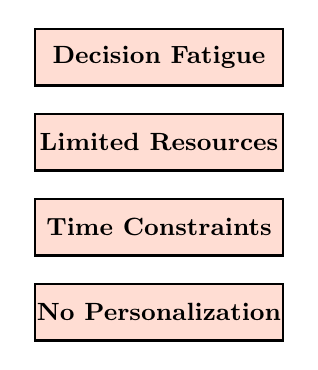
\begin{tikzpicture}[scale=0.9]
            % Problem boxes
            \draw[fill=Warning!20, thick] (0,0) rectangle (3.5,0.8);
            \node at (1.75, 0.4) {\small \textbf{Decision Fatigue}};
            
            \draw[fill=Warning!20, thick] (0,-1.2) rectangle (3.5,-0.4);
            \node at (1.75, -0.8) {\small \textbf{Limited Resources}};
            
            \draw[fill=Warning!20, thick] (0,-2.4) rectangle (3.5,-1.6);
            \node at (1.75, -2.0) {\small \textbf{Time Constraints}};
            
            \draw[fill=Warning!20, thick] (0,-3.6) rectangle (3.5,-2.8);
            \node at (1.75, -3.2) {\small \textbf{No Personalization}};
        \end{tikzpicture}
        
        \column{0.48\textwidth}
        \centering
        \textcolor{Accent}{\Large \textbf{OUR SOLUTION}}
        
        \vspace{0.8cm}
        
        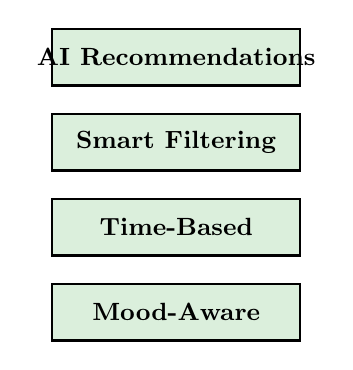
\begin{tikzpicture}[scale=0.9]
            % Solution boxes
            \draw[fill=Accent!20, thick] (0,0) rectangle (3.5,0.8);
            \node at (1.75, 0.4) {\small \textbf{AI Recommendations}};
            
            \draw[fill=Accent!20, thick] (0,-1.2) rectangle (3.5,-0.4);
            \node at (1.75, -0.8) {\small \textbf{Smart Filtering}};
            
            \draw[fill=Accent!20, thick] (0,-2.4) rectangle (3.5,-1.6);
            \node at (1.75, -2.0) {\small \textbf{Time-Based}};
            
            \draw[fill=Accent!20, thick] (0,-3.6) rectangle (3.5,-2.8);
            \node at (1.75, -3.2) {\small \textbf{Mood-Aware}};
        \end{tikzpicture}
    \end{columns}
\end{frame}

% ============================================================
% SLIDE 3: KEY FEATURES
% ============================================================
\begin{frame}{Key Features}
    \vspace*{0.3cm}
    
    \begin{tikzpicture}[
        feature/.style={
            rectangle, 
            rounded corners=5pt, 
            inner sep=12pt, 
            text width=2.8cm,
            text centered,
            font=\small\bfseries,
            shadow={shadow xshift=2pt, shadow yshift=-2pt}
        }
    ]
        % Row 1
        \node[feature, fill=Primary!30] (f1) at (0, 5) {🎭 Mood\\Filtering};
        \node[feature, fill=Secondary!30] (f2) at (3.2, 5) {🥘 Ingredient\\Matching};
        \node[feature, fill=Accent!30] (f3) at (6.4, 5) {⏱️ Time-\\Aware};
        
        % Row 2
        \node[feature, fill=Primary!30] (f4) at (0, 2.8) {❤️ Favorites\\System};
        \node[feature, fill=Secondary!30] (f5) at (3.2, 2.8) {📱 Offline\\Capable};
        \node[feature, fill=Accent!30] (f6) at (6.4, 2.8) {👥 User\\Profiles};
        
        % Row 3
        \node[feature, fill=Primary!30] (f7) at (1.6, 0.6) {📤 Recipe\\Upload};
        \node[feature, fill=Secondary!30] (f8) at (4.8, 0.6) {⚙️ Admin\\Controls};
    \end{tikzpicture}
    
    \vspace*{2.5cm}
    \centering
    \small \textcolor{gray}{All features designed for intuitive user experience}
\end{frame}

% ============================================================
% SLIDE 4: TECHNOLOGY STACK
% ============================================================
\begin{frame}{Technology Stack}
    \vspace*{0.5cm}
    
    \begin{columns}[T]
        \column{0.32\textwidth}
        \centering
        \textcolor{Primary}{\textbf{\large Frontend}}
        
        \vspace{0.5cm}
        
        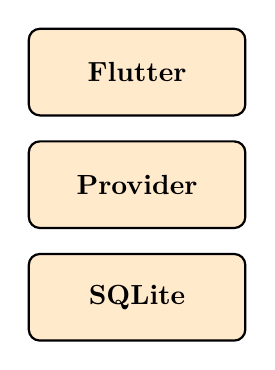
\begin{tikzpicture}[scale=1.1]
            \draw[fill=Primary!20, thick, rounded corners] (0,0) rectangle (2.5,1);
            \node at (1.25, 0.5) [align=center] {\textbf{Flutter}};
            
            \draw[fill=Primary!20, thick, rounded corners] (0,-1.3) rectangle (2.5,-0.3);
            \node at (1.25, -0.8) [align=center] {\textbf{Provider}};
            
            \draw[fill=Primary!20, thick, rounded corners] (0,-2.6) rectangle (2.5,-1.6);
            \node at (1.25, -2.1) [align=center] {\textbf{SQLite}};
        \end{tikzpicture}
        
        \column{0.32\textwidth}
        \centering
        \textcolor{Secondary}{\textbf{\large Backend}}
        
        \vspace{0.5cm}
        
        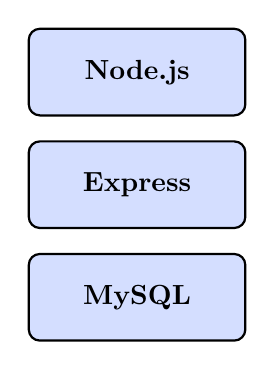
\begin{tikzpicture}[scale=1.1]
            \draw[fill=Secondary!20, thick, rounded corners] (0,0) rectangle (2.5,1);
            \node at (1.25, 0.5) [align=center] {\textbf{Node.js}};
            
            \draw[fill=Secondary!20, thick, rounded corners] (0,-1.3) rectangle (2.5,-0.3);
            \node at (1.25, -0.8) [align=center] {\textbf{Express}};
            
            \draw[fill=Secondary!20, thick, rounded corners] (0,-2.6) rectangle (2.5,-1.6);
            \node at (1.25, -2.1) [align=center] {\textbf{MySQL}};
        \end{tikzpicture}
        
        \column{0.32\textwidth}
        \centering
        \textcolor{Accent}{\textbf{\large DevOps}}
        
        \vspace{0.5cm}
        
        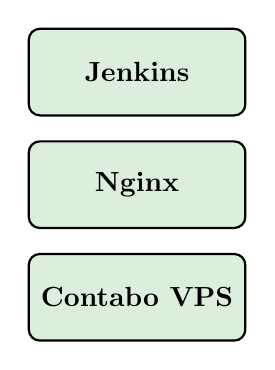
\begin{tikzpicture}[scale=1.1]
            \draw[fill=Accent!20, thick, rounded corners] (0,0) rectangle (2.5,1);
            \node at (1.25, 0.5) [align=center] {\textbf{Jenkins}};
            
            \draw[fill=Accent!20, thick, rounded corners] (0,-1.3) rectangle (2.5,-0.3);
            \node at (1.25, -0.8) [align=center] {\textbf{Nginx}};
            
            \draw[fill=Accent!20, thick, rounded corners] (0,-2.6) rectangle (2.5,-1.6);
            \node at (1.25, -2.1) [align=center] {\textbf{Contabo VPS}};
        \end{tikzpicture}
    \end{columns}
\end{frame}

% ============================================================
% SLIDE 5: SYSTEM ARCHITECTURE
% ============================================================
\begin{frame}{System Architecture}
    \vspace*{0.3cm}
    
    \begin{tikzpicture}[scale=0.95, thick]
        % Mobile Client
        \draw[fill=Primary!30, thick, rounded corners=8pt] (1.5, 8) rectangle (4, 9);
        \node at (2.75, 8.5) [align=center] {\textbf{📱 Flutter}\\Client};
        
        % Cloud symbol
        \draw[fill=Secondary!20, thick, rounded corners=8pt] (6, 8) rectangle (8.5, 9);
        \node at (7.25, 8.5) [align=center] {\textbf{☁️ API}\\Gateway};
        
        % Backend Services
        \draw[fill=Secondary!30, thick, rounded corners=8pt] (0.5, 5.5) rectangle (2.8, 6.5);
        \node at (1.65, 6) {\textbf{Auth}};
        
        \draw[fill=Secondary!30, thick, rounded corners=8pt] (3.2, 5.5) rectangle (5.5, 6.5);
        \node at (4.35, 6) {\textbf{Recipe}};
        
        \draw[fill=Secondary!30, thick, rounded corners=8pt] (5.8, 5.5) rectangle (8.1, 6.5);
        \node at (6.95, 6) {\textbf{Favorites}};
        
        % Database
        \draw[fill=Accent!30, thick, rounded corners=8pt] (3, 2.5) rectangle (5.5, 3.5);
        \node at (4.25, 3) [align=center] {\textbf{MySQL}\\Database};
        
        % Cache
        \draw[fill=Accent!30, thick, rounded corners=8pt] (6.2, 2.5) rectangle (8.5, 3.5);
        \node at (7.35, 3) [align=center] {\textbf{Redis}\\Cache};
        
        % Arrows
        \draw[->, thick, Primary, shorten >=3pt, shorten <=3pt] (4, 8) -- (7.2, 9);
        \draw[->, thick, Primary, shorten >=3pt, shorten <=3pt] (7.2, 8) -- (4, 8);
        
        \draw[->, thick, Secondary, shorten >=3pt, shorten <=3pt] (4.35, 5.5) -- (4.35, 3.5);
        \draw[->, thick, Secondary, shorten >=3pt, shorten <=3pt] (5.5, 6) -- (6.2, 3);
        
        % Labels
        \node[above, font=\tiny, text=gray] at (5.6, 8.5) {REST API};
        \node[left, font=\tiny, text=gray] at (4.2, 4.5) {Queries};
    \end{tikzpicture}
    
    \vspace*{1cm}
    \centering
    \small \textcolor{gray}{Layered architecture with Repository pattern}
\end{frame}

% ============================================================
% SLIDE 6: USER FLOW - MOOD FILTERING
% ============================================================
\begin{frame}{User Flow: Mood-Based Recipe Discovery}
    \vspace*{0.5cm}
    
    \begin{tikzpicture}[
        node distance=2cm,
        scale=0.85,
        every node/.style={rectangle, rounded corners=5pt, text centered, font=\small\bfseries}
    ]
        % Step 1
        \node[fill=Primary!30, text width=2.2cm] (step1) at (0, 6) {Select\\Mood};
        
        % Step 2
        \node[fill=Secondary!30, text width=2.2cm] (step2) at (3, 6) {Choose\\Ingredients};
        
        % Step 3
        \node[fill=Accent!30, text width=2.2cm] (step3) at (6, 6) {Set Time\\Limit};
        
        % Step 4
        \node[fill=Primary!30, text width=2.2cm] (step4) at (9, 6) {View\\Results};
        
        % Arrows
        \draw[->, thick, color=Primary, shorten >=3pt, shorten <=3pt] (step1) -- (step2);
        \draw[->, thick, color=Secondary, shorten >=3pt, shorten <=3pt] (step2) -- (step3);
        \draw[->, thick, color=Accent, shorten >=3pt, shorten <=3pt] (step3) -- (step4);
        
        % Icons below
        \node[below=0.5cm of step1, font=\Large, inner sep=0] {🎭};
        \node[below=0.5cm of step2, font=\Large, inner sep=0] {🥘};
        \node[below=0.5cm of step3, font=\Large, inner sep=0] {⏱️};
        \node[below=0.5cm of step4, font=\Large, inner sep=0] {✨};
        
        % Mood Emotions
        \node[below=2.2cm of step1, fill=Primary!20, text width=2.2cm, text height=1.2cm] {Happy • Sad • Energetic • Comfort • Healthy • Quick • Light};
    \end{tikzpicture}
    
    \vspace*{1.5cm}
    
    \begin{center}
        \includegraphics[width=0.7\textwidth]{../Diagrams/sequence\ diagram\ recipe\ by\ mood.png}
    \end{center}
\end{frame}

% ============================================================
% SLIDE 7: DESIGN PATTERNS & ARCHITECTURE
% ============================================================
\begin{frame}{Design Patterns \& Architecture}
    \vspace*{0.3cm}
    
    \begin{columns}[T]
        \column{0.48\textwidth}
        \centering
        \textcolor{Primary}{\textbf{\large Design Patterns}}
        
        \vspace{0.5cm}
        
        \begin{itemize}
            \item \textbf{🏗️ Provider Pattern}\\State management
            \vspace{0.3cm}
            \item \textbf{🗂️ Repository Pattern}\\Data abstraction
            \vspace{0.3cm}
            \item \textbf{👤 Singleton Pattern}\\Shared instances
            \vspace{0.3cm}
            \item \textbf{🏭 Factory Pattern}\\Object creation
        \end{itemize}
        
        \column{0.48\textwidth}
        
        \centering
        \includegraphics[width=0.95\textwidth]{../Diagrams/classdiagram.png}
    \end{columns}
\end{frame}

% ============================================================
% SLIDE 8: DEPLOYMENT & DEVOPS
% ============================================================
\begin{frame}{Deployment \& DevOps Pipeline}
    \vspace*{0.5cm}
    
    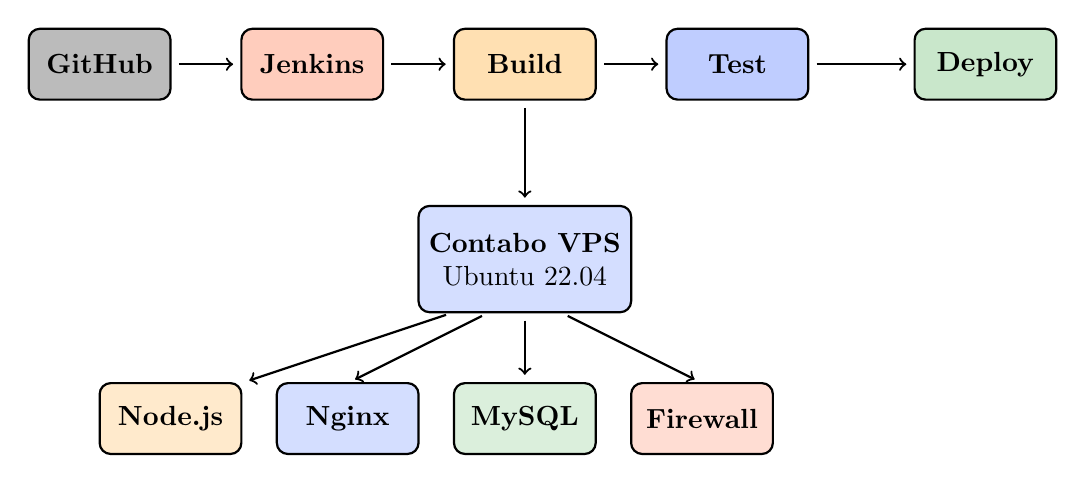
\begin{tikzpicture}[scale=0.9, thick]
        % GitHub
        \draw[fill=DarkBg!30, thick, rounded corners] (0, 5) rectangle (2, 6);
        \node at (1, 5.5) {\textbf{GitHub}};
        
        % Jenkins
        \draw[fill=Warning!30, thick, rounded corners] (3, 5) rectangle (5, 6);
        \node at (4, 5.5) {\textbf{Jenkins}};
        
        % Build
        \draw[fill=Primary!30, thick, rounded corners] (6, 5) rectangle (8, 6);
        \node at (7, 5.5) {\textbf{Build}};
        
        % Test
        \draw[fill=Secondary!30, thick, rounded corners] (9, 5) rectangle (11, 6);
        \node at (10, 5.5) {\textbf{Test}};
        
        % Arrows top
        \draw[->, thick, shorten >=3pt, shorten <=3pt] (2, 5.5) -- (3, 5.5);
        \draw[->, thick, shorten >=3pt, shorten <=3pt] (5, 5.5) -- (6, 5.5);
        \draw[->, thick, shorten >=3pt, shorten <=3pt] (8, 5.5) -- (9, 5.5);
        \draw[->, thick, shorten >=3pt, shorten <=3pt] (11, 5.5) -- (12.5, 5.5);
        
        % Deploy
        \draw[fill=Accent!30, thick, rounded corners] (12.5, 5) rectangle (14.5, 6);
        \node at (13.5, 5.5) {\textbf{Deploy}};
        
        % VPS
        \draw[fill=Secondary!20, thick, rounded corners] (5.5, 2) rectangle (8.5, 3.5);
        \node at (7, 2.75) [align=center] {\textbf{Contabo VPS}\\Ubuntu 22.04};
        
        % Services
        \draw[fill=Primary!20, thick, rounded corners] (1, 0) rectangle (3, 1);
        \node at (2, 0.5) {\textbf{Node.js}};
        
        \draw[fill=Secondary!20, thick, rounded corners] (3.5, 0) rectangle (5.5, 1);
        \node at (4.5, 0.5) {\textbf{Nginx}};
        
        \draw[fill=Accent!20, thick, rounded corners] (6, 0) rectangle (8, 1);
        \node at (7, 0.5) {\textbf{MySQL}};
        
        \draw[fill=Warning!20, thick, rounded corners] (8.5, 0) rectangle (10.5, 1);
        \node at (9.5, 0.5) {\textbf{Firewall}};
        
        % Arrows down
        \draw[->, thick, shorten >=3pt, shorten <=3pt] (7, 5) -- (7, 3.5);
        \draw[->, thick, shorten >=3pt, shorten <=3pt] (6, 2) -- (3, 1);
        \draw[->, thick, shorten >=3pt, shorten <=3pt] (6.5, 2) -- (4.5, 1);
        \draw[->, thick, shorten >=3pt, shorten <=3pt] (7, 2) -- (7, 1);
        \draw[->, thick, shorten >=3pt, shorten <=3pt] (7.5, 2) -- (9.5, 1);
    \end{tikzpicture}
    
    \vspace*{1cm}
    \centering
    \small \textcolor{gray}{\textbf{99.8\% Uptime} | CI/CD Automation | Real-time Monitoring}
\end{frame}

% ============================================================
% SLIDE 9: TESTING & METRICS
% ============================================================
\begin{frame}{Testing \& Quality Metrics}
    \vspace*{0.5cm}
    
    \begin{columns}[T]
        \column{0.48\textwidth}
        \centering
        \textcolor{Primary}{\textbf{\large Test Coverage}}
        
        \vspace{0.8cm}
        
        \begin{tikzpicture}[scale=1.0]
            % Pie chart representation
            \draw[fill=Accent!60, thick] (0,0) -- (0,2) arc[start angle=90, end angle=262.2, radius=2] -- cycle;
            \node at (-0.7, 0.5) {\small \textbf{48.5\%}};
            
            \draw[fill=Primary!60, thick] (0,0) -- (0,2) arc[start angle=262.2, end angle=90, radius=2] -- cycle;
            \node at (1.2, 1.0) {\small \textbf{51.5\%}};
            
            % Legend
            \node[below=1.5cm of current bounding box.south, text width=3cm, align=center, font=\small] {
                \textcolor{Accent}{●} Unit Tests\\
                \textcolor{Primary}{●} Integration Tests
            };
        \end{tikzpicture}
        
        \column{0.48\textwidth}
        \centering
        \textcolor{Secondary}{\textbf{\large Performance}}
        
        \vspace{0.5cm}
        
        \begin{tabularx}{0.95\textwidth}{|l|c|}
            \hline
            \rowcolor{Secondary!20}
            \textbf{Metric} & \textbf{Target} \\
            \hline
            Recipe Load Time & \textcolor{Accent}{\textbf{<2s}} \\
            \hline
            API Response & \textcolor{Accent}{\textbf{<500ms}} \\
            \hline
            Database Query & \textcolor{Accent}{\textbf{<300ms}} \\
            \hline
            Uptime & \textcolor{Accent}{\textbf{99.8\%}} \\
            \hline
        \end{tabularx}
    \end{columns}
\end{frame}

% ============================================================
% SLIDE 10: CONCLUSION & FUTURE ROADMAP
% ============================================================
\begin{frame}{Conclusion \& Future Roadmap}
    \vspace*{0.5cm}
    
    \begin{columns}[T]
        \column{0.48\textwidth}
        \centering
        \textcolor{Primary}{\textbf{\large Achievements}}
        
        \vspace{0.5cm}
        
        \begin{itemize}
            \item ✨ Fully functional cross-platform app
            \vspace{0.3cm}
            \item 🔐 Secure authentication system
            \vspace{0.3cm}
            \item 📱 Offline-first architecture
            \vspace{0.3cm}
            \item ⚡ Fast, responsive UI
            \vspace{0.3cm}
            \item 🚀 Automated deployment
            \vspace{0.3cm}
            \item 📊 Comprehensive testing
        \end{itemize}
        
        \column{0.48\textwidth}
        \centering
        \textcolor{Secondary}{\textbf{\large Future Enhancements}}
        
        \vspace{0.5cm}
        
        \begin{itemize}
            \item 🤖 AI-powered recommendations
            \vspace{0.3cm}
            \item 🌍 Multi-language support
            \vspace{0.3cm}
            \item 📊 Advanced analytics
            \vspace{0.3cm}
            \item 🔔 Smart notifications
            \vspace{0.3cm}
            \item 🎯 Nutrition tracking
            \vspace{0.3cm}
            \item 👨‍👩‍👧‍👦 Social sharing
        \end{itemize}
    \end{columns}
    
    \vspace*{1.5cm}
    \centering
    \Large \textcolor{Primary}{\textbf{Making meal planning accessible, enjoyable, and efficient}}
\end{frame}

% ============================================================
% THANK YOU SLIDE
% ============================================================
\begin{frame}[plain]
    \begin{tikzpicture}[remember picture, overlay]
        \fill[color=Primary!5] (current page.south west) rectangle (current page.north east);
        \fill[color=Secondary!10] (current page.north west) -- (current page.north east) -- 
              ($(current page.north east)!0.4!(current page.south east)$) -- 
              ($(current page.north west)!0.4!(current page.south west)$) -- cycle;
    \end{tikzpicture}
    
    \centering
    \vspace*{2cm}
    
    {\Huge \textbf{\textcolor{Primary}{Thank You!}}}\\[1cm]
    
    {\Large \textcolor{Secondary}{Questions?}}\\[2cm]
    
    \includegraphics[width=0.2\textwidth]{../assets/logo/PICK\ MY\ DISH.png}\\[1.5cm]
    
    {\small \faGithub\ \href{https://github.com/Kynmmarshall/Pick-My-Dish}{GitHub Repository}}\\
    {\small \faGlobe\ \href{https://pickmydish.duckdns.org}{Live Application}}\\[1.5cm]
    
    {\footnotesize \textcolor{gray}{ICT University - SEN3140 | December 2025}}
\end{frame}

\end{document}
